\documentclass{beamer}
\usetheme{Warsaw}

\usepackage{amsfonts} % math symobls
\usepackage{amsthm}
\usepackage[utf8]{inputenc}
\usepackage{polski}
\usepackage{graphics}
\usepackage{verbatim}
\usepackage{tikz}
\usetikzlibrary{arrows}
\usetikzlibrary{calc}

\newtheorem{tw}{Twierdzenie}
\newtheorem{lem}{Lemat}
\newtheorem{df}{Definicja}
\newtheorem{obs}{Obserwacja}  

\newcommand{\emp}[1]{\textcolor{blue}{\textit{#1}}}
\newcommand{\red}[1]{\textcolor{red}{#1}}
\newcommand{\tuple}[2]{\langle #1 , #2 \rangle}

\title{A Fully Dynamic Reachability Algorithm for Directed Graphs}
\subtitle{with an Almost Linear Update Time}
\author{Michał Karpiński}
\date{8 stycznia, 2013}

\begin{document}

\begin{frame}[plain]
  \titlepage
\end{frame}

\begin{frame}{Specyfika problemu (wersja statyczna)}
Dane: 

\begin{itemize}
\item graf skierowany $G$ oraz wierzchołki $u,v \in V(G)$
\end{itemize}

Wynik:

\begin{itemize}
\item Odpowiedź na pytanie: czy w $G$ istnieje ścieżka z $u$ do $v$?
\end{itemize}

\vspace{0.5cm}

\begin{center}
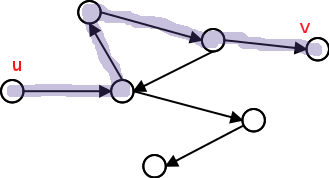
\includegraphics[scale=0.5]{img/Diagram1.png}
\end{center}

\end{frame}

\begin{frame}{Specyfika problemu (wersja dynamiczna)}

Różnica: graf $G$ zmienia się w czasie!


\vspace{0.5cm}

Cel: zbudowanie struktury danych wspierającej operacje:
\begin{itemize}
\item \emp{Update} - aktualizuje graf
\item \emp{Query} - odpowiada na pytanie o osiągalność
\end{itemize}
\end{frame}

\begin{frame}{Silnie spójne składowe (SSS)}

\begin{df}
{\bf Silnie spójna składowa} grafu skierowanego $G$ to taki maksymalny podgraf $H$, a jednocześnie jego spójna składowa, taka, że pomiędzy każdymi dwoma jej wierzchołkami istnieje ścieżka.
\end{df}

\begin{center}
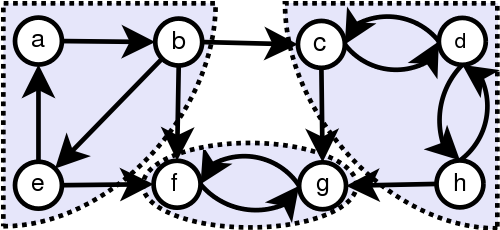
\includegraphics[scale=0.5]{img/Scc.png}
\end{center}

\end{frame}

\begin{frame}{Silnie spójne składowe (SSS)}
Problem: mając dany graf $G$, czy $u,v \in V(G)$ należą do tej samej silnie spójnej składowej?

\vspace{0.5cm}

\begin{itemize}
\item wersja statyczna - proste
\item wersja dynamiczna - zaraz się okaże :)
\end{itemize}

\vspace{0.5cm}

\begin{block}{Uwaga}
Struktura rozwiązująca problem dynamiczny SSS jest kluczem do utworzenia struktury rozwiązującej problem dynamiczny osiągalności w grafie skierowanym!
\end{block}

\end{frame}

\begin{frame}{Porządane procedury}

\begin{itemize}
\item \emp{Insert(E')} - tworzy nową \red{wersję grafu}, początkowo identyczną z poprzednią \red{wersją}, w której dodajemy zbiór krawędzi $E'$
\item \emp{Delete(E')} - usuwa zbiór krawędzi $E'$ ze \red{{\bf wszystkich} wersji grafu}
\item \emp{Query(u,v,i)} - sprawdza, czy $u$ i $v$ należą do wspólnego komponentu w $i$-tej wersji grafu
\end{itemize}

\end{frame}

\begin{frame}{Porządane procedury}
\begin{block}{Bardziej formalnie}
Algorytm zachowuje komponenty grafów $G_1,G_2 \cdots G_t$, gdzie $t$ jest liczbą operacji \emp{Insert} wykonaną do tej pory. Definiujemy $G_i=\tuple{V}{E_i}$ jako graf utworzony po $i$-tej operacji \emp{Insert}.
\end{block}

\begin{block}{Uproszczenie}
Zakładamy, że graf początkowy $G_0=\tuple{V}{E_0}$ jest grafem bez krawędzi, czyli $E_0 = \phi$. 
\end{block}
\end{frame}


%%% PIERWSZA PARTIA
%\begin{comment}
\begin{frame}{Przykład}

\begin{columns}
\begin{column}<1->{0.25\textwidth}
\begin{center}$G_0$\end{center}
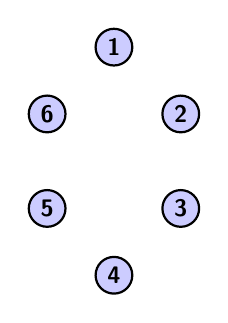
\begin{tikzpicture}[->,>=stealth',shorten >=1pt,auto,node distance=2cm,
  thick,main node/.style={circle,fill=blue!20,draw,font=\sffamily\Large\bfseries}]

  \node[main node,scale=0.6] (1) {1};
  \node[main node,scale=0.6] (2) [below right of=1] {2};
  \node[main node,scale=0.6] (3) [below of=2] {3};
  \node[main node,scale=0.6] (4) [below left of=3] {4};
  \node[main node,scale=0.6] (6) [below left of=1] {6};
  \node[main node,scale=0.6] (5) [below of=6] {5};
\end{tikzpicture}
\end{column}

\begin{column}<2->{0.25\textwidth}
\begin{center}$G_1$\end{center}
\begin{tikzpicture}[->,>=stealth',shorten >=1pt,auto,node distance=2cm,
  thick,main node/.style={circle,fill=blue!20,draw,font=\sffamily\Large\bfseries}]

  \fill<3->[fill=blue,fill opacity=0.4] ($(6.west)+(-0.25,0.4)$) -- ($(6.east)+(0.25,0.4)$) -- ($(5.east)+(0.25,-0.4)$) -- ($(5.west)+(-0.25,-0.4)$) -- cycle; 

  \node[main node,scale=0.6] (1) {1};
  \node[main node,scale=0.6] (2) [below right of=1] {2};
  \node[main node,scale=0.6] (3) [below of=2] {3};
  \node[main node,scale=0.6] (4) [below left of=3] {4};
  \node[main node,scale=0.6] (6) [below left of=1] {6};
  \node[main node,scale=0.6] (5) [below of=6] {5};

  \path
    (3) edge node [left] {} (4)
    (5) edge [bend left] node[left] {} (6)
    (6) edge [bend left] node[left] {} (5)
        edge node[right] {} (1);
\end{tikzpicture}
\end{column}

\begin{column}<4->{0.25\textwidth}
\begin{center}$G_2$\end{center}
\begin{tikzpicture}[->,>=stealth',shorten >=1pt,auto,node distance=2cm,
  thick,main node/.style={circle,fill=blue!20,draw,font=\sffamily\Large\bfseries}]

\fill<5->[fill=green,fill opacity=0.4] ($(6.west)+(-0.25,0.4)$) -- ($(6.east)+(0.25,0.4)$) -- ($(3.east)+(0.25,0.4)$) -- ($(3.east)+(0.25,-1.25)$) -- ($(5.west)+(-0.25,-1.25)$) -- cycle; 

  \node[main node,scale=0.6] (1) {1};
  \node[main node,scale=0.6] (2) [below right of=1] {2};
  \node[main node,scale=0.6] (3) [below of=2] {3};
  \node[main node,scale=0.6] (4) [below left of=3] {4};
  \node[main node,scale=0.6] (6) [below left of=1] {6};
  \node[main node,scale=0.6] (5) [below of=6] {5};

  \path
    (3) edge node [left] {} (4)
    (5) edge [bend left] node[left] {} (6)
        edge node [right] {} (3)
    (4) edge [bend right] node [left] {} (6)
    (6) edge [bend left] node[left] {} (5)
        edge node[right] {} (1);
\end{tikzpicture}
\end{column}

\begin{column}<6->{0.25\textwidth}
\begin{center}$G_3$\end{center}
\begin{tikzpicture}[->,>=stealth',shorten >=1pt,auto,node distance=2cm,
  thick,main node/.style={circle,fill=blue!20,draw,font=\sffamily\Large\bfseries}]

\fill<7->[fill=red,fill opacity=0.4] ($(6.west)+(-0.25,0.4)$) -- ($(2.east)+(0.25,0.4)$) -- ($(3.east)+(0.25,-1.20)$) -- ($(5.west)+(-0.25,-1.20)$) -- cycle;

  \node[main node,scale=0.6] (1) {1};
  \node[main node,scale=0.6] (2) [below right of=1] {2};
  \node[main node,scale=0.6] (3) [below of=2] {3};
  \node[main node,scale=0.6] (4) [below left of=3] {4};
  \node[main node,scale=0.6] (6) [below left of=1] {6};
  \node[main node,scale=0.6] (5) [below of=6] {5};

  \path
    (2) edge node {} (3)
    (3) edge node [left] {} (4)
    (5) edge [bend left] node[left] {} (6)
        edge node [right] {} (3)
    (4) edge [bend right] node [left] {} (6)
    (6) edge [bend left] node[left] {} (5)
        edge node[right] {} (1)
        edge node[right] {} (2);
\end{tikzpicture}
\end{column}
\end{columns}

\only<8>{\vspace{0.5cm}\begin{obs}
Każdy komponent z $G_i$ jest albo kompenentem z $G_{i-1}$, albo sumą pewnych komponentów z $G_{i-1}$.
\end{obs}}

\onslide<9->{\vspace{0.2cm}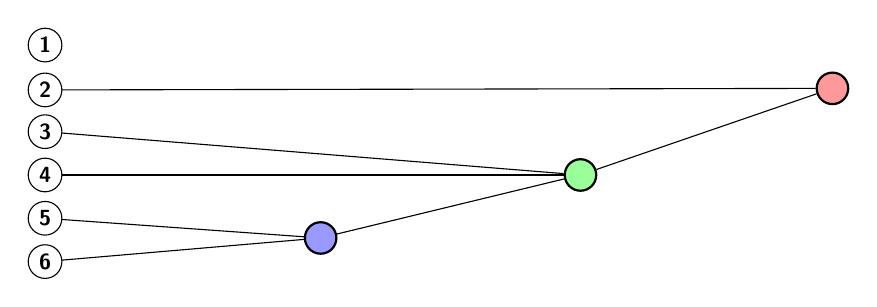
\begin{tikzpicture}[main node/.style={circle,fill=white!20,draw,font=\sffamily\Large\bfseries}]
  \node[thick,circle,fill=blue,fill opacity=0.4,minimum width=0.4cm,draw] (g1) at (3.5,-2.45) {};
  \node[thick,circle,fill=green,fill opacity=0.4,minimum width=0.4cm,draw] (g2) at (6.8,-1.65) {} edge (g1);
  \node[thick,circle,fill=red,fill opacity=0.4,minimum width=0.4cm,draw] (g3) at (10,-0.55) {} edge (g2);
  \node[main node,scale=0.55] (1) at (0,0) {1};
  \node[main node,scale=0.55] (2) at (0,-0.57) {2} edge (g3);
  \node[main node,scale=0.55] (3) at (0,-1.1) {3} edge (g2);
  \node[main node,scale=0.55] (4) at (0,-1.65) {4} edge (g2);
  \node[main node,scale=0.55] (5) at (0,-2.2) {5} edge (g1);
  \node[main node,scale=0.55] (6) at (0,-2.75) {6} edge (g1);

\end{tikzpicture}}

\end{frame}
%\end{comment} bulke wroclawska, proszek do prania
%%%%%%%%%%%%%%%%%%%%%%%%%%%%%%%%%%


\begin{frame}{Lowest Common Ancestor}
\begin{obs}
Jeśli (w jakiś sposób) będziemy przechowywać las komponentów dla ciągu $G_0,G_1 \cdots G_t$, to operacja \emp{Query} może być zredukowana do zapytania \emp{LCA} na tym lesie.
\end{obs}

\begin{block}{Przypomnienie}
Wiadomo, że można wykonać preprocessing na lasie o liczbie wierzchołków \alert{$O(n)$}, w czasie \alert{$O(n)$} tak, aby zapytania \emp{LCA} wykonywać w czasie stałym \alert{$O(1)$}. Żródła:

\vspace{0.1cm}
{\small\textit{D. Harel and R. Tarjan. Fast algorithms for finding nearest common ancestros. SIAM Journal on Computing, 13:338-355, 1984.}}

\vspace{0.1cm}
{\small\textit{B. Shieber and U. Vishkin. On finding lowest common ancestors: Simplification and parallelization. SIAM Journal on Computing, 17:1253-1262, 1988.}}
\end{block}
\end{frame}

\begin{frame}{Dynamic edge partitioning}
\begin{df}
Mamy dane zbiory krawędzi $E_1 \subseteq E_2 \subseteq \cdots \subseteq E_t$. Dla każdego $i=1\dots t$, \textbf{dynamiczny zbiór krawędzi} $H_i$ grafu $G_i$ jest zdefiniowany jako:

\vspace{0.4cm}
{\small $H_i = \{(u,v)\in E_i | Query(u,v,i) \wedge (\neg Query(u,v,i-1) \vee (u,v) \notin E_{i-1})\}$}

\vspace{0.4cm}
oraz

\vspace{0.4cm}
{\small $H_{t+1} = E_t \setminus \cup^t_{i=1}H_i$}

\end{df}
\end{frame}

%%%% DRUGA PARTIA
\begin{comment}
\begin{frame}{Przykład}

\begin{columns}
\begin{column}{0.25\textwidth}
\begin{center}$G_0$\end{center}
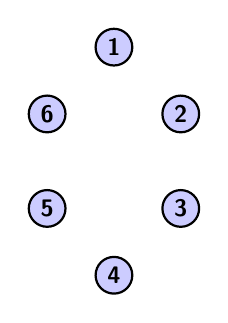
\begin{tikzpicture}[->,>=stealth',shorten >=1pt,auto,node distance=2cm,
  thick,main node/.style={circle,fill=blue!20,draw,font=\sffamily\Large\bfseries}]

  \node[main node,scale=0.6] (1) {1};
  \node[main node,scale=0.6] (2) [below right of=1] {2};
  \node[main node,scale=0.6] (3) [below of=2] {3};
  \node[main node,scale=0.6] (4) [below left of=3] {4};
  \node[main node,scale=0.6] (6) [below left of=1] {6};
  \node[main node,scale=0.6] (5) [below of=6] {5};
\end{tikzpicture}
\end{column}

\begin{column}{0.25\textwidth}
\begin{center}$G_1$\end{center}
\begin{tikzpicture}[->,>=stealth',shorten >=1pt,auto,node distance=2cm,
  thick,main node/.style={circle,fill=blue!20,draw,font=\sffamily\Large\bfseries}]

  \fill[fill=blue,fill opacity=0.4] ($(6.west)+(-0.25,0.4)$) -- ($(6.east)+(0.25,0.4)$) -- ($(5.east)+(0.25,-0.4)$) -- ($(5.west)+(-0.25,-0.4)$) -- cycle; 

  \node[main node,scale=0.6] (1) {1};
  \node[main node,scale=0.6] (2) [below right of=1] {2};
  \node[main node,scale=0.6] (3) [below of=2] {3};
  \node[main node,scale=0.6] (4) [below left of=3] {4};
  \node[main node,scale=0.6] (6) [below left of=1] {6};
  \node[main node,scale=0.6] (5) [below of=6] {5};

  \path
    (3) edge node [left] {} (4)
    (5) edge [line width=1.5pt,orange!70,bend left] node[left] {} (6)
    (6) edge [line width=1.5pt,orange!70,bend left] node[left] {} (5)
        edge node[right] {} (1);
\end{tikzpicture}
\end{column}

\begin{column}{0.25\textwidth}
\begin{center}$G_2$\end{center}
\begin{tikzpicture}[->,>=stealth',shorten >=1pt,auto,node distance=2cm,
  thick,main node/.style={circle,fill=blue!20,draw,font=\sffamily\Large\bfseries}]

\fill[fill=green,fill opacity=0.4] ($(6.west)+(-0.25,0.4)$) -- ($(6.east)+(0.25,0.4)$) -- ($(3.east)+(0.25,0.4)$) -- ($(3.east)+(0.25,-1.25)$) -- ($(5.west)+(-0.25,-1.25)$) -- cycle; 

  \node[main node,scale=0.6] (1) {1};
  \node[main node,scale=0.6] (2) [below right of=1] {2};
  \node[main node,scale=0.6] (3) [below of=2] {3};
  \node[main node,scale=0.6] (4) [below left of=3] {4};
  \node[main node,scale=0.6] (6) [below left of=1] {6};
  \node[main node,scale=0.6] (5) [below of=6] {5};

  \path
    (3) edge [line width=1.5pt,orange!70] node [left] {} (4)
    (5) edge [bend left] node[left] {} (6)
        edge [line width=1.5pt,orange!70] node [right] {} (3)
    (4) edge [line width=1.5pt,orange!70,bend right] node [left] {} (6)
    (6) edge [bend left] node[left] {} (5)
        edge node[right] {} (1);
\end{tikzpicture}
\end{column}

\begin{column}{0.25\textwidth}
\begin{center}$G_3$\end{center}
\begin{tikzpicture}[->,>=stealth',shorten >=1pt,auto,node distance=2cm,
  thick,main node/.style={circle,fill=blue!20,draw,font=\sffamily\Large\bfseries}]

\fill[fill=red,fill opacity=0.4] ($(6.west)+(-0.25,0.4)$) -- ($(2.east)+(0.25,0.4)$) -- ($(3.east)+(0.25,-1.20)$) -- ($(5.west)+(-0.25,-1.20)$) -- cycle;

  \node[main node,scale=0.6] (1) {1};
  \node[main node,scale=0.6] (2) [below right of=1] {2};
  \node[main node,scale=0.6] (3) [below of=2] {3};
  \node[main node,scale=0.6] (4) [below left of=3] {4};
  \node[main node,scale=0.6] (6) [below left of=1] {6};
  \node[main node,scale=0.6] (5) [below of=6] {5};

  \path
    (2) edge [line width=1.5pt,orange!40] node {} (3)
    (3) edge node [left] {} (4)
    (5) edge [bend left] node[left] {} (6)
        edge node [right] {} (3)
    (4) edge [bend right] node [left] {} (6)
    (6) edge [bend left] node[left] {} (5)
        edge node[right] {} (1)
        edge [line width=1.5pt,orange!40] node[right] {} (2);
\end{tikzpicture}
\end{column}
\end{columns}

\vspace{0.3cm}
\begin{center}Do zbioru $H_{t+1}=H_4$ należy krawędź $\{6,1\}$.\end{center}

\end{frame}
\end{comment}
%%%%%%%%%%

\begin{frame}{Dynamic set partitioning}
\begin{itemize}
\item $E_t = \cup^{t+1}_{i=1}H_i$
\item $H_i \cap H_j = \phi$ dla każdego $1 \leq i < j \leq t+1$
\item Zbiór $H_i$ jest złożony ze wszystkich krawędzi łączących dwa różne komponenty w $G_{i-1}$ lub takich, które nie znajdują się w $G_{i-1}$, ale łączą dwa różne komponenty w $G_i$.
\end{itemize}

\begin{block}{}
Taki podział jest \textbf{dynamiczny} ze względu na to, że każda zmiana w lesie komponentów może powodować przeniesienie krawędzi z $H_i$ do $H_j$, dla $i < j$.
\end{block}
\end{frame}

\begin{frame}{Union-Find}
Prosta struktura do pamiętania zbiorów rozłącznych.
\begin{itemize}
\item \emp{Find(a)} - zwraca reprezentanta zbioru $a$. 
\item \emp{Union(Find(a),Find(b))} - łączy zbiory, zawierające $a$ i $b$
\end{itemize}
\begin{block}{Przypomnienie}
Łączny czas wykonania $m$ operacji \emp{Union} i \emp{Find} na zbiorach rozłącznych, zawierających w sumie $n$ elementów, jest równy $O(m\cdot\alpha(m,n))$, gdzie $\alpha$ jest odwrotnością funkcji Ackermanna.
\end{block}
\end{frame}

\begin{frame}{Algorytm}
Struktury:
\begin{itemize}
\item \emp{parent} - tablica przechowująca dla każdego wierzchołka w lesie, wskaźnik do jego ojca
\item \emp{version} - tablica przechowująca dla każdego wierzchołka w której wersji grafu po raz pierwszy pojawił się komponent związany z tym wierzchołkiem
\end{itemize}
\end{frame}

\begin{frame}{Algorytm - procedury}
\begin{center}
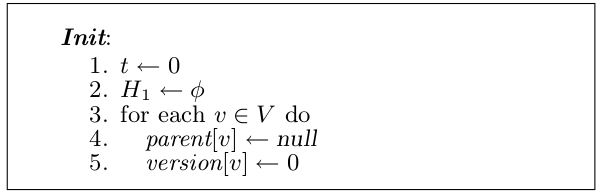
\includegraphics[scale=0.4]{img/Init.png}
\end{center}

\begin{obs}
Dwa wierzchołki $u$ i $v$ należą do tego samego komponentu w $G_i$ wtedy i tylko wtedy, gdy wersja ich najniższego wspólnego przodka jest mniejsza bądź równa $i$.
\end{obs}

\begin{center}
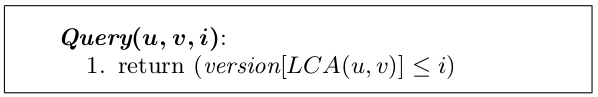
\includegraphics[scale=0.4]{img/Query.png}
\end{center}
\end{frame}

\begin{frame}{Algorytm - procedury}
\begin{center}
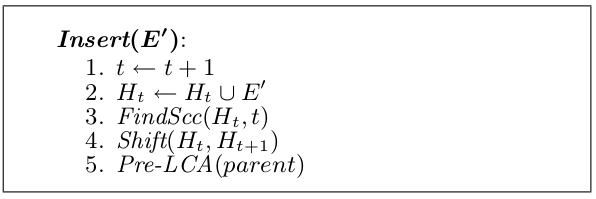
\includegraphics[scale=0.4]{img/Insert.png}
\end{center}

\begin{itemize}
\item \emp{FindScc($H_t$,$t$)} - aktualizuje las komponentów
\item \emp{Shift($H_t$,$H_{t+1}$)} - wydziela zbiór $H_{t+1}$ z $H_t$
\item \emp{Pre-LCA(parent)} - preprocesing dla zapytań LCA
\end{itemize}
\end{frame}

%TRZECIA PRATIA
%\begin{comment}
\begin{frame}{Przykład}

\begin{columns}
\begin{column}{0.25\textwidth}
\begin{center}$G_0$\end{center}
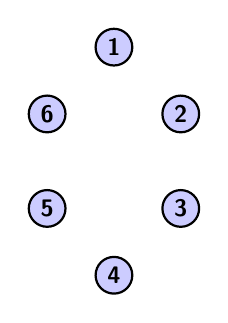
\begin{tikzpicture}[->,>=stealth',shorten >=1pt,auto,node distance=2cm,
  thick,main node/.style={circle,fill=blue!20,draw,font=\sffamily\Large\bfseries}]

  \node[main node,scale=0.6] (1) {1};
  \node[main node,scale=0.6] (2) [below right of=1] {2};
  \node[main node,scale=0.6] (3) [below of=2] {3};
  \node[main node,scale=0.6] (4) [below left of=3] {4};
  \node[main node,scale=0.6] (6) [below left of=1] {6};
  \node[main node,scale=0.6] (5) [below of=6] {5};
\end{tikzpicture}
\end{column}

\begin{column}{0.25\textwidth}<3->
\begin{center}$G_1$\end{center}
\begin{tikzpicture}[->,>=stealth',shorten >=1pt,auto,node distance=2cm,
  thick,main node/.style={circle,fill=blue!20,draw,font=\sffamily\Large\bfseries}]

  \fill<4->[fill=blue,fill opacity=0.4] ($(6.west)+(-0.25,0.4)$) -- ($(6.east)+(0.25,0.4)$) -- ($(5.east)+(0.25,-0.4)$) -- ($(5.west)+(-0.25,-0.4)$) -- cycle; 

  \node[main node,scale=0.6] (1) {1};
  \node[main node,scale=0.6] (2) [below right of=1] {2};
  \node[main node,scale=0.6] (3) [below of=2] {3};
  \node[main node,scale=0.6] (4) [below left of=3] {4};
  \node[main node,scale=0.6] (6) [below left of=1] {6};
  \node[main node,scale=0.6] (5) [below of=6] {5};

  \path
    (3) edge node [left] {} (4)
    (5) edge [bend left] node[left] {} (6)
    (6) edge [bend left] node[left] {} (5)
        edge node[right] {} (1);
\end{tikzpicture}
\end{column}
\end{columns}

\vspace{0.2cm}

\onslide<2->\emp{Insert($\{ (5,6),(6,5),(6,1),(3,4) \}$):}
\begin{itemize}
\item<3-> wstawiamy nowe krawędzie. $H_1 = \{ (5,6),(6,5),(6,1),(3,4) \}$
\item<4-> \emp{FindScc} znajduje nowe komponenty i tworzy nowe wierzchołki w lesie
\item<5-> \emp{Shift} dzieli $H_1$ na $H_1= \{ (5,6),(6,5)\}$ i $H_2=\{(6,1),(3,4)\}$
\end{itemize}

\end{frame}
%\end{comment}


\begin{frame}{Algorytm - procedury}
\begin{center}
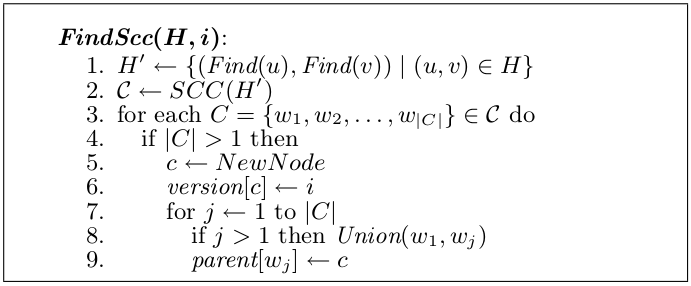
\includegraphics[scale=0.4]{img/FindScc.png}
\end{center}

\begin{center}
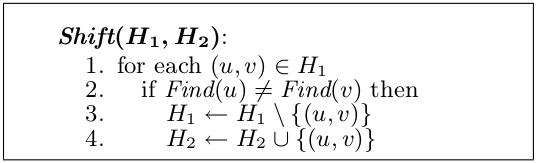
\includegraphics[scale=0.4]{img/Shift.png}
\end{center}
\end{frame}

\begin{frame}{Algorytm - procedury}
\begin{center}
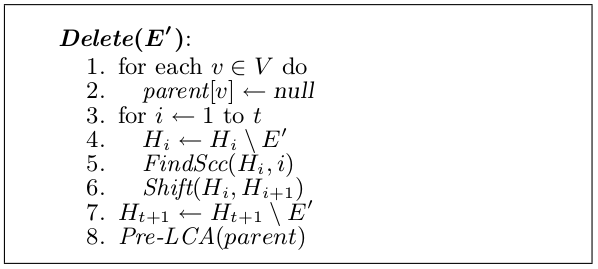
\includegraphics[scale=0.4]{img/Delete.png}
\end{center}
\end{frame}

\end{document}
